\begin{center}
    \textbf{\titlePageWorkType~№\titlePageWorkNumber~\titlePageWorkPart}
\end{center}

\textbf{Тема}: <<\titlePageTopic>>

%\textbf{Цель работы}: 

\begin{center}
    \textbf{Ход работы}:
\end{center}

Написать ассемблерную вставку, реализующую следующую обработку строки: согласно варианту.
Оформить ее в виде отдельной функции.
Реализовать данную обработку строки также в виде функции на С++.
Сравнить быстродействие обоих вариантов.
В отчете отразить выводы.
Для разработки использовать MS Visual Studio.

\textbf{Варианты}:
\begin{enumerate}
    \item[1.] Перевернуть строку.
    \item[2.] Поменять четные символы с нечетными.
    \item[3.] Даны 4 строки. Поменять 1-ю с 3-ей, 2-ю с 4-й.
    \item[4.] Даны 2 строки. Совместить четные символы одной строки с нечентными другой.
    \item[5.] Даны 2 строки. Совместить половину строки 1 с половиной строки 2.
    \item[6.] Нечетные символы заменить на +.
    \item[7.] Совместить 2-е строки. Совпадающие символы заменить на 0.
    \item[8.] Сместить все символы на 1-н вперед циклично.
    \item[9.] Перевернуть две половины строки.
    \item[10.] Сместить все символы на 1-н назад циклично.
    \item[11.] Заменить пробелы на символ табуляции.
    \item[12.] Заменить пробелы на символ табуляции.
    \item[13.] Удалить повторяющиеся пробелы, также пробелы в начале и в конце строки.
\end{enumerate}

Пример функции с ассемблерной вставкой (С++ Visual Studio): 

\begin{lstlisting}[
    name=Пример assembler'ной вставки,
    basicstyle=\ttfamily\scriptsize,
]
    int f()
    {
        __asm
        {
            mov eax, 1
            int 3
        }
        return 0;
    }
\end{lstlisting}

\newpage

\begin{center}
    \textbf{Вариант 6}
\end{center}

\textbf{Условие}:
Нечетные символы заменить на +.

\textbf{Решение}:

\lstinputlisting[
    language=C++,
    basicstyle=\ttfamily\scriptsize,
]
{../../src/option6/src/main.cpp}

\newpage

\begin{lstlisting}[
    name=Console log,
    basicstyle=\ttfamily\scriptsize,
]
Test change string on C++
str = "Hello, World!"
str = "H+l+o+ +o+l+!"

Test change string on Assembler
str = "Hello, World!"
str = "H+l+o+ +o+l+!"

           1              0.000000000000        C++
           1              0.000000000000        Assembler
          10              0.000000000000        C++
          10              0.000000000000        Assembler
         100              0.000000000000        C++
         100              0.000000000000        Assembler
        1000              0.000000000000        C++
        1000              0.001000000000        Assembler
       10000              0.001000000000        C++
       10000              0.001000000000        Assembler
      100000              0.023000000000        C++
      100000              0.028000000000        Assembler
     1000000              0.211000000000        C++
     1000000              0.218000000000        Assembler
    10000000              1.982000000000        C++
    10000000              2.085000000000        Assembler
\end{lstlisting}

%\lstinputlisting[
%    language=Python,
%    basicstyle=\ttfamily\scriptsize,
%]
%{../../src/writeGraph/src/main.py}

\begin{figure}[!htp]
    \centering
    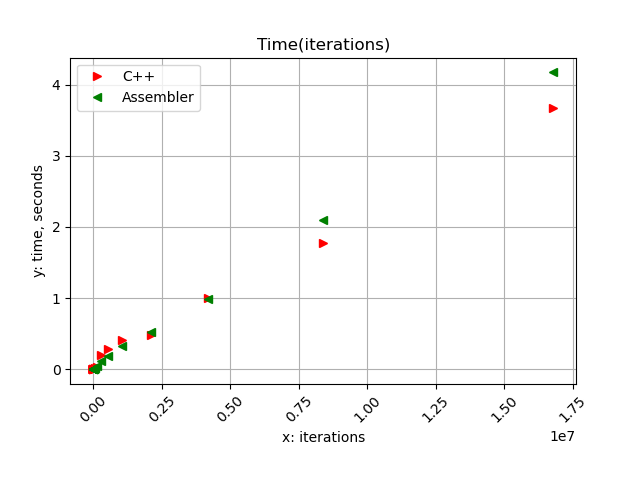
\includegraphics[]
    {../_INCLUDES/option6.png}
    \caption{Зависимосте времени от итерации (С++/Assembler)}
\end{figure}